\documentclass{article}
\usepackage[utf8]{inputenc}
\usepackage{kotex}
\usepackage{graphicx}
\usepackage{verbatim}
\usepackage{placeins}
\usepackage{geometry}

\geometry{
    a4paper,
    left=30mm,
    right=30mm,
    top=30mm,
    bottom=40mm
}

\title{자료구조 HW4 ShortestPath}
\author{C211123 이준선}
\date{\today}

\begin{document}
\maketitle
\tableofcontents
\listoffigures
\listoftables
\newpage

\section{개요}
본 보고서는 미로의 입구에서부터 출구까지의 최단 경로를 찾는 ShortestPath 함수에 대한 설명이다. BFS($Breadth First Search$, 너비우선탐색) 알고리즘과 백트래킹 기법을 사용하였다.

\section{BFS와 Backtracking}
\subsection{너비우선탐색 BFS}
BFS는 가까운 트리나 그래프 등의 노드들을 우선적으로 탐색하는 기법이다. 즉 DFS($Depth First Search$, 깊이우선탐색)과 비교할 때, DFS는 노드들을 깊게 탐색하는 반면 BFS는 넓게 탐색한다.

트리를 예시로 들 경우, 우선 같은 레벨의 노드(트리)를 우선적으로 방문하여 탐색한 후, 이후 다음 레벨의 트리에 진입해 탐색을 이어간다. DFS는 우선적으로 레벨의 깊이를 높여나가는 것과 대조적이다. DFS는 재귀적으로 구현 가능하지만, 자칫 모든 노드들을 전부 방문하게 될 수도 있다. 반면 BFS는 queue(큐)를 이용하며, DFS보다 구현 난이도는 높지만 DFS보다 근소하게 시간 복잡도 면에서 성능 우위를 가진다고 알려져 있다. 한편 BFS는 자칫 검색해야 할 경우의 수가 증가할 수록, DFS에 비해 공간복잡도가 기하급수적으로 늘어나기에 overflow 에러가 쉽게 발생할 수가 있다. 실제로 이번 과제를 진행하며 shortestPath() 함수를 구현할 때도, Visual Studio에서 stack 저장 공간에 대한 오버플로우 경고를 보냈다.\footnote{BFS에 의한 직접적인 오버플로우 경고가 아닌, stack의 과도한 메모리 사용을 시도하는 것에 대한 오류이긴 했으나, BFS를 진행하기 위한 공간 할당이므로 간접적인 영향을 확인할 수 있다.} 즉 DFS, BFS는 장단점이 있으며 상황에 맞춰 적절한 알고리즘을 선택하는 게 중요하다.
\begin{figure} [h]
    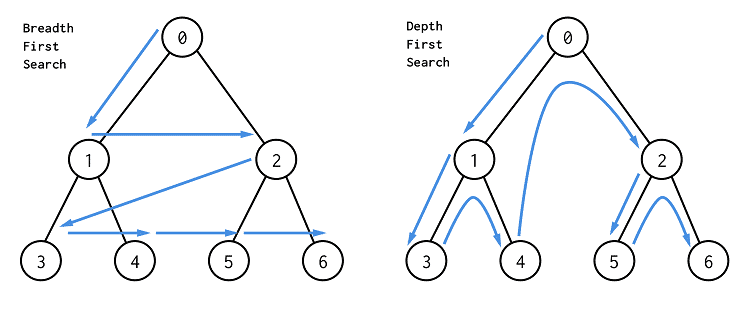
\includegraphics[width = \textwidth]{images_vagabondms_post_037c243c-108a-49c6-ae6a-abb3673532ca_image.png}
    \caption{DFS와 BFS의 차이\footnotemark}
    \label{fig:DFS_BFS}
\end{figure}
\footnotetext{김민석. “DFS vs BFS.” Velog.Io, 5 Mar. 2021, velog.io/@vagabondms/DFS-vs-BFS.}
한편 그래프에서는 한 정점에 인접한, 또는 직접적으로 연결된 정점들을 먼저 모두 찾아 queue에 저장한 후, 다음 정점들을 찾아가는 방식이라고 볼 수 있다.
\subsection{백트래킹 Backtracking}
백트래킹은 이번 shortestPath 구현에서 핵심이 된 기법으로, 각 경로에 대한 이전 정보를 저장하여, 출구에서 입구까지의 최단 경로를 역으로 추적하는 기법을 사용했다. map을 사용하여 현재 노드(current)와 이전 노드의 정보를 저장하였다.

\section{ShortestPath 코드 설명}
\subsection{코드 전문}
\lstset{language=C++}
\textbf{shortestPath()}
\begin{verbatim}}
/*********
* function : ShortestPath
* parameters
*	m : 행
*	p : 열
* description :
*	m * n 미로의 최단 경로를 찾는다. queue를 이용하고, bfs 알고리즘을 사용한다.
*	현재 위치에서 움직일 수 있는 모든 경우의 수를 inqueue한다.
*	queue를 차례로 dequeue하여, 각 dequeue한 position마다 새로이 다시금 움직일 수 있는 모든 경우의 수를 inqueue한다.
*	이를 반복하다가, exit()에 reach하면, 그것이 shortest path가 된다.
*	상세한 설명은 latex 참조
*	https://youtu.be/ZuHW4fS60pc <- 해당 영상 알고리즘을 참고하였음.
********/
void ShortestPath(const int m, const int p)
{
    	const int numberOfEntireNode = m * p; ///> 전체 노드 개수
    	int visitedNode = 0; ///> 방문한 노드 개수
    	// stack 안에다가 큰 배열 사용 시 C6262 overflow error를 일으킬 가능성이 있어서, 배열은 엥간하면 동적 배열로 heap에다가 저장.
    	bool** mark_short = new bool* [MAXSIZE + 1]; ///> 그냥 mark는 path함수가 사용했으므로, Shortest가 사용할 mark_short 표시
    	for (int i = 0; i < MAXSIZE + 1; i++) {
        		mark_short[i] = new bool[MAXSIZE + 1]();
    	}
    
    	bool** mark_frontier = new bool* [MAXSIZE + 1]; ///> frontier queue에 이미 추가된 장소를 표시. 
    	// 이미 queue에 대기중이라면 애써 또 추가할 필요 없다
    	for (int i = 0; i < MAXSIZE + 1; i++) {
        		mark_frontier[i] = new bool[MAXSIZE + 1]();
    	}
    	Position current(1, 1, E); ///> 시작 위치로 초기화한 현재 위치
    	queue<Position> frontier; ///> 여기에 다음으로 이동할 정보들을 담는다
    	map<Position, Position> visited; ///> 방문 장소, 직전 노드들의 정보 담는다
    
    	Position forward = current;
    
    	map<Position, Position> mothers; ///> frontier를 추가할 때, 추가된 forward에 대한 mother=current 로 지정
    	mothers.insert(make_pair(current, current)); // 시작 위치에 대한 mother value는 시작 위치 그 자신
    	Position exit(m, p, N); ///> 탈출 노드
    	frontier.push(current);
    
    	while (!frontier.empty()) {
        		current = frontier.front();
        		visitedNode++; // 방문 노드 추가
        		mark_short[current.x][current.y] = 1; // 노드 방문했다고 표시남김
        
        		// if reached exit
        		if (current == exit) {
            			visited.insert(make_pair(current, mothers[current]));
            			backtracking(visited, current);
            			cout << endl << "#nodes visited = " << visitedNode;
            			cout << " out of " << numberOfEntireNode << endl;
            
            			// 끝내기 전에 동적 할당 해제
            			for (int i = 0; i < MAXSIZE + 1; i++) {
            				delete[] mark_short[i];
            				delete[] mark_frontier[i];
            			}
            
            			delete[] mark_short; delete[] mark_frontier;
            			return;
        		}
        		for (int d = 0; d < 8; d++) {
            			forward = moveDir(current, d);
            
            			if (maze[forward.x][forward.y] != 1 && mark_short[forward.x][forward.y] != 1) {
                				if (mark_frontier[forward.x][forward.y] != 1) {
                					frontier.push(forward);
                					mark_frontier[forward.x][forward.y] = 1; 
                					// frontier에 추가되었으므로, 추가되었다고 표시함
                					mothers.insert(make_pair(forward, current)); 
                					// forward의 mother=current를 저장
                				}
            			}
        		}
        		visited.insert(make_pair(current, mothers[current]));
        
        		frontier.pop();
    	}
    
    	cout << "No path in maze." << endl;
    	// 끝내기 전에 동적 할당 해제
    	for (int i = 0; i < MAXSIZE + 1; i++) {
        		delete[] mark_short[i];
        		delete[] mark_frontier[i];
    	}
    
    	delete[] mark_short; delete[] mark_frontier;
}
\end{verbatim}

\textbf{backtracking()}
\begin{verbatim}}
void backtracking(map<Position, Position>& moves, Position& trackStartPoint) {
    	stack<Position> list;
    	Position cur = trackStartPoint;
    	while (cur != moves[cur]) {
        		list.push(cur);
        		cur = moves[cur];
    	}
    	list.push(cur); // 시작 위치까지 집어넣어줌
    
    	while (!list.empty()) {
        		cout << list.top(); list.pop();
    	}
}
\end{verbatim}

\textbf{moveDir()}
\begin{verbatim}
/***********
* 이동을 담당하는 함수, cur에다가 현재 위치, dir에 방향을 담으면
* 그 방향으로 한 칸 이동한 위치가 반환됨
***********/
Position moveDir(const Position& cur, int dir) {
    	Position forward;
    	forward.x = cur.x + movea[dir].a;
    	forward.y = cur.y + movea[dir].b;
    	forward.dir = dir;
    
    	return forward;
}
\end{verbatim}

\textbf{operator==, operator != for Position compare}
\begin{verbatim}}
bool operator==(const Position& a, const Position& b) {
    	if (a.x == b.x && a.y == b.y) {
        		return true;
    	}
    	else return false;
}
bool operator!=(const Position& a, const Position& b) {
    	if (a.x != b.x || a.y != b.y) {
        		return true;
    	}
    	else return false;
}
\end{verbatim}

\textbf{struct Position}
\begin{verbatim}}
/*********
* 현재 자기가 어디에 있고, 다음에 어디에 갈 건지를 포함하는 구조체
* x, y좌표가 있고
* dir은 다음에 갈 방향
* 왔던 길은 push, 만약에 막혀서 돌아가는 거면 pop을 한다.
********/
struct Position {
	Position(int xx = 0, int yy = 0, int dd = 0) : x(xx), y(yy), dir(dd) {}
	int x, y, dir;

	// map의 key값으로 이용할 거라서, 정렬을 위한 비교 연산자 정의해줘야 함.
	bool operator< (const Position& tem) const {
    		if (x > tem.x) {
        			return true;
    		}
    		else if (x < tem.x) {
        			return false;
    		}
    		else {
        			if (y > tem.y) {
            				return true;
        			}
        			else if (y < tem.y) {
            				return false;
        			}
        			else return false;
    		}
    	}
};
\end{verbatim}
\subsection{moveDir() 함수}
moveDir() 함수는 이동을 직관적으로 보이기 위한 함수로, parameter에 현재 위치(cur), 그리고 방향을 담으면 해당 방향으로 이동한 결과인 Position struct를 반환한다.
새로 만들어진 Position의 방향은 parameter로 전달된 dir과 일치하게 만들었다. 다만 shortestPath()에서 Position struct의 방향 값은 크게 신경쓰지 않는데, 이전 노드의 좌표를 참고해서 backtracking을 할 뿐, 다음에 탐색할 방향을 Position struct가 저장하진 않기 때문이다. 따라서 Path() 함수 말고 shortestPath() 만 사용할 것이라면, 약간의 코드 수정과 함께 Position struct의 dir 은 지워도 상관 없다.
\subsection{struct Position}
Position에서 operator$<$을 정의한 것을 볼 수 있는데, 이는 map$<$Position, Position$>$형 매핑 자료형을 사용하기 때문이다. map은 key값을 기준으로 내부적으로 정렬되는데, 이때 키값에 일반적인 int, double같은 값이 들어간다면 상관이 없으나, 비교 연산자가 정의되지 않은 struct를 key값으로 집어넣었기에 operator$<$을 정의해야 한다.\\
한편 비교연산자 operator$<$은 tight한 논리연산을 수행해야 하며, 즉 값이 $>$일 때 뿐만이 아니라 $=$일 때도 false를 반환해야 한다. 한편 operator$<$에서도 dir에 대한 비교 연산은 진행하지 않는다.
\subsection{operator==, operator!=}
Position의 비교 연산을 위한 연산자 정의이다. 두 포지션의 x, y 값이 같다면 $==$, 다르다면 $!=$을 리턴한다.\\
dir은 비교하지 않는다. dir이 달라도 위치가 같다면 두 Position은 같은 것으로 취급한다.

\\
이상으로 구현의 편의성을 위해 필요한 몇 가지 기능들을 정의하였다. 이하부터는 실제로 알고리즘의 기반이 되는 shortestPath()와 backtracking() 함수를 살펴보겠다.
\subsection{shortestPath() 함수}

\FloatBarrier
\begin{figure} [h]
    \centering
    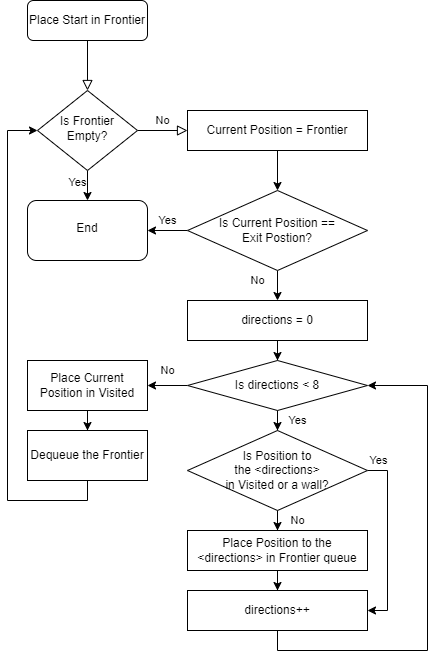
\includegraphics[height = 15cm]{flow chart.drawio.png}
    \caption{shortestPath() 함수의 순서도}
    \label{fig:flowChart}
\end{figure}
\FloatBarrier
shortestPath() 함수의 기본적인 알고리즘 순서도(flow chart)는 Figure \ref{fig:flowChart}를 통해 확인할 수 있다.

shortestPath() 함수는 너비 우선 탐색(BFS)를 사용하였으며, 가까운 노드를 Queue형 자료형인 Frontier에 저장한다. 한편 방문한 노드는 Visited에 저장하며, 이때 backtracking을 위해 Visited에 저장할 때, 바로 직전 노드 정보를 같이 저장한다. 이를 위해, Visited는 map형 자료형으로 선언한다. mapping을 통해 방문한 노드 current와 바로 직전 노드 정보를 1대 1로 매칭시킨다. 순서도를 따라가며 코드를 살펴보자.

\begin{enumerate}
    \item 필요한 변수들 준비
    \begin{verbatim}
    bool** mark_short = new bool* [MAXSIZE + 1];
	for (int i = 0; i < MAXSIZE + 1; i++) {
    		mark_short[i] = new bool[MAXSIZE + 1]();
	}

	bool** mark_frontier = new bool* [MAXSIZE + 1];
	for (int i = 0; i < MAXSIZE + 1; i++) {
    		mark_frontier[i] = new bool[MAXSIZE + 1]();
	}

	Position current(1, 1, E);

	queue<Position> frontier;

	map<Position, Position> visited;

	Position forward = current;

	map<Position, Position> mothers; 
	mothers.insert(make_pair(current, current)); 

	Position exit(m, p, N);
    \end{verbatim}
    \textbf{mark$_$short} 배열은 방문한 Position을 체크하기 위한 2차원 배열이다. \textbf{mark$_$frontier} 배열은 frontier에 저장할 Position을 저장하는 배열로써, frontier에 중복으로  Position이 추가되는 것을 막기 위한 배열이다.\\
    위 두 배열이 상당히 큰 용량의 메모리 공간을 사용하기에, 정적 할당을 통해 stack 저장 영역에 배열을 관리하는 것보다 동적 할당을 통해 heap 영역에 배열을 저장하였다. 정적으로 배열을 선언할 경우, stack 저장공간이 부족하다는 경고가 발생할 수 있다.
    
    \textbf{current}는 현재 위치를 나타내는 Position이다. 시작 위치인 (1, 1)로 초기화되며, 방향은 임의의 값인 E로 초기화하였다\footnote{다시 한 번 강조하지만, shortestPath() 함수에서는 Position.dir 변수를 활용하지 않는다.}. 
    
    \textbf{frontier}는 앞으로 탐색할 위치를 저장하는 queue이다. BFS에 따라, current를 기준으로 이웃한 8방향의 Position중 이동 가능한 Postition을 저장한다.
    
    \textbf{visited}는 방문한 Position을 저장하는 map이다. key에는 방문한 current Position, 그리고 value값에는 current를 안내한 직전 mother Position을 담는다.\\
    예를 들어, (2, 2)에서 BFS를 통해 (3, 2)를 Frontier에 담았고, 이후 (3, 2)로 이동하여 current = (3, 2)가 되었다고 하자. 이때는 (2, 2)가 (3, 2)를 소개하였으므로 mother = (2, 2)가 된다. 반대로 current Position은 mother의 `자식 Position'이라 할 수 있다. 하나의 current Position은 오직 하나의 mother Position만 가지지만, 하나의 mother Position은 여러 개의 자식 Position을 가질 수 있다. \\ 이 정보는 이후 최단 경로를 찾기 위한 backtracking에 유용하게 쓰인다.
    
    \textbf{forward}는 current의 mother Position을 저장하기 위한 Position이다.
    
    \textbf{mothers}는 현재 current 노드의 mother Position을 저장하기 위한 map이다. mothers는 visited를 저장하기 위해 사용되는 임시 저장 공간이다.
    
    \textbf{exit}은 출구 Position이다.
    \item Place Start in Frontier
    \begin{verbatim}
    frontier.push(current);
    \end{verbatim}
    start Position인 current Position을 frontier에 추가한다.
    \item Current Position = Frontier
    \begin{verbatim}
        current = frontier.front();
		mark_short[current.x][current.y] = 1; // 노드 방문했다고 표시남김
    \end{verbatim}
    frontier queue에서 하나를 뽑아내 current에 저장한다. 그리고 해당 current 위치에 방문했다고 표시를 남긴다.
    \item if current Position == exit Position
    \begin{verbatim}
    if (current == exit) {
			visited.insert(make_pair(current, mothers[current]));
			backtracking(visited, current);
			cout << endl << "#nodes visited = " << visitedNode << " out of ";
			cout << numberOfEntireNode << endl;

			// 끝내기 전에 동적 할당 해제
			for (int i = 0; i < MAXSIZE + 1; i++) {
    				delete[] mark_short[i];
    				delete[] mark_frontier[i];
			}

			delete[] mark_short; delete[] mark_frontier;
			return;
	}
    \end{verbatim}
    current와 exit이 같으면 미로의 탈출구를 찾았으므로, 더 이상의 탐색을 진행하지 않고 저장한다. 현재 위치 (exit Position)을 visited에 저장한다. 그리고 backtracking() 함수를 호출하여 최단 경로를 출력한다. 한편 동적할당한 mark$_$short 배열과 mark$_$frontier 배열을 해제한다.
    \item Searching frontier
    \begin{verbatim}
    for (int d = 0; d < 8; d++) {
    		forward = moveDir(current, d);
    
    		if (maze[forward.x][forward.y] != 1 && mark_short[forward.x][forward.y] != 1) {
    				if (mark_frontier[forward.x][forward.y] != 1) {
        					frontier.push(forward);
        					mark_frontier[forward.x][forward.y] = 1; // frontier에 추가되었으므로, 추가되었다고 표시함
        					mothers.insert(make_pair(forward, current)); // forward의 mother=current를 저장
    				}
    		}
    }
    \end{verbatim}
    d = N(0)부터 8방향을 검사한다. moveDir() 함수를 통해 이동한 Position을 forward에 저장하고, forward가 벽(1)이 아니고 이전에 방문한 적이 없으며, forward Position이 이미 frontier에 대기 중이 아니라면 frontier에 forward를 추가한다. 그리고 forward의 부모 Position을 mothers mapping을 통해 저장한다.
    \item dequeue frontier
    \begin{verbatim}
		visited.insert(make_pair(current, mothers[current]));
		frontier.pop();
    \end{verbatim}
    visited map에 current Position과, current Position의 mother Position을 저장한다. 이후 frontier를 dequeue하고, 다음 탐색을 이어간다.
\end{enumerate}

\subsection{backtracking() 함수}
backtracking() 함수는 알고리즘을 완성하는 아름다운 기법이다. 백트래킹의 기본적인 원리는 이전 노드 (mother Position)을 추적하는 가장 최단 경로를 찾아간다는 데 있다.
\FloatBarrier
\begin{figure} [h]
    \centering
    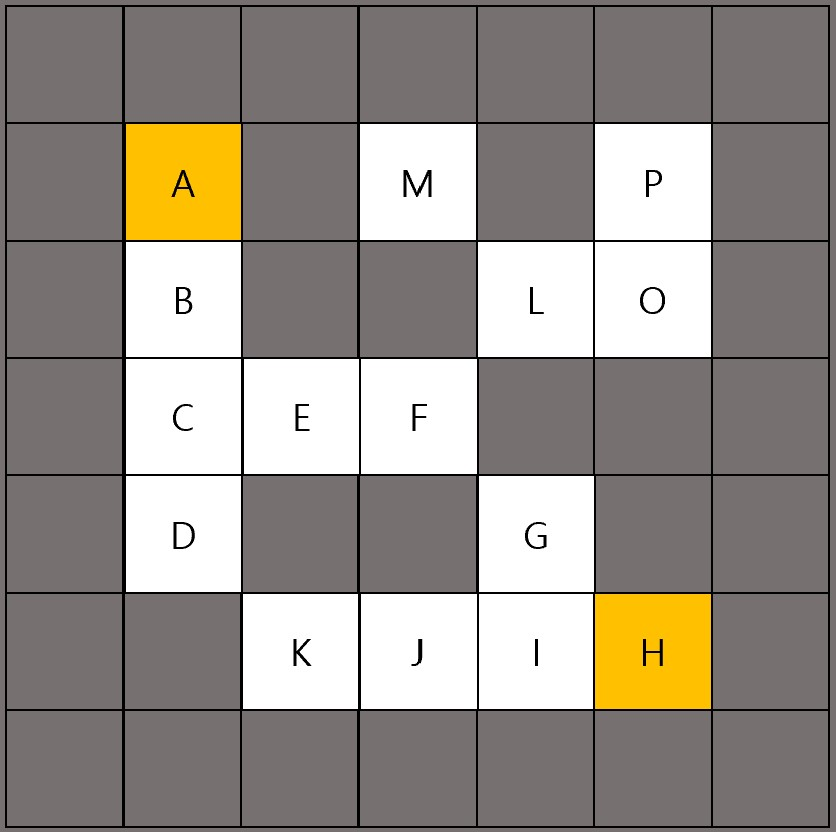
\includegraphics{mazePicture.jpg}
    \caption{예시 미로}
    \label{fig:mazePic}
\end{figure}
\FloatBarrier
\FloatBarrier
\begin{table}[h]
\centering
\caption{예시 미로Figure\ref{fig:mazePic}에 대한 BFS 서칭 결과}
\label{table:tb1}
\begin{tabular}{|c|c|}
\noalign{\smallskip}\noalign{\smallskip}\hline
current & mother \\ \hline
A       & A      \\ \hline
B       & A      \\ \hline
E       & B      \\ \hline
F       & E      \\ \hline
D       & E      \\ \hline
C       & B      \\ \hline
L       & F      \\ \hline
G       & F      \\ \hline
K       & D      \\ \hline
P       & L      \\ \hline
O       & L      \\ \hline
M       & L      \\ \hline
H       & G      \\ \hline
\end{tabular}
\end{table}
\FloatBarrier
Figure \ref{fig:mazePic}에서 A는 시작위치, H는 탈출위치를 나타낸다. Table \ref{table:tb1}은 Figure \ref{fig:mazePic}의 BFS 탐색 결과이다. backtracking 과정은 다음과 같이 이루어진다. 먼저 출구인 H의 mother Position인 G로 간다. G의 mother인 F, F에서 E, E에서 B, B에서 A로 간다. A의 mother은 A 자신이므로 A가 시작점이 된다. 즉 Figure \ref{fig:mazePic}의 최단 경로는 A $\rightarrow$ B $\rightarrow$ E $\rightarrow$ F $\rightarrow$ G $\rightarrow$ H 이다. 이 과정을 그대로 코드로 옮겨보면 아래와 같다.

\begin{verbatim}
void backtracking(map<Position, Position>& moves, Position& trackStartPoint) {
    	stack<Position> list;
    	Position cur = trackStartPoint;
    	while (cur != moves[cur]) {
        		list.push(cur);
        		cur = moves[cur];
    	}
    	list.push(cur); // 시작 위치까지 집어넣어줌
    
    	while (!list.empty()) {
        		cout << list.top(); list.pop();
    	}
}
\end{verbatim}
backtracking의 과정을 그대로 뒤집어서 출력할 것이니 stack을 이용한다. 첫 번째 인자에는 visited, 두 번째 인자에는 백트래킹을 시작할 위치(출구 Position)을 받는다. trackStartPoint로부터 cur의 mother Position이 cur 자신이 될 때까지 백트래킹한 결과를 stack에 저장한다. 그리고 자신이 될 때가 바로 시작점이다. 저장된 스택을 다시 출력하면 끝난다.

\end{document}
